\appendix
\renewcommand*{\appendixpagename}{Anhang}
\renewcommand*{\appendixtocname}{Anhang}
\appendixpage 
\addappheadtotoc
\chapter{Aufbau der Wetterstation} 
%\begin{figure}[h]
%\centering
%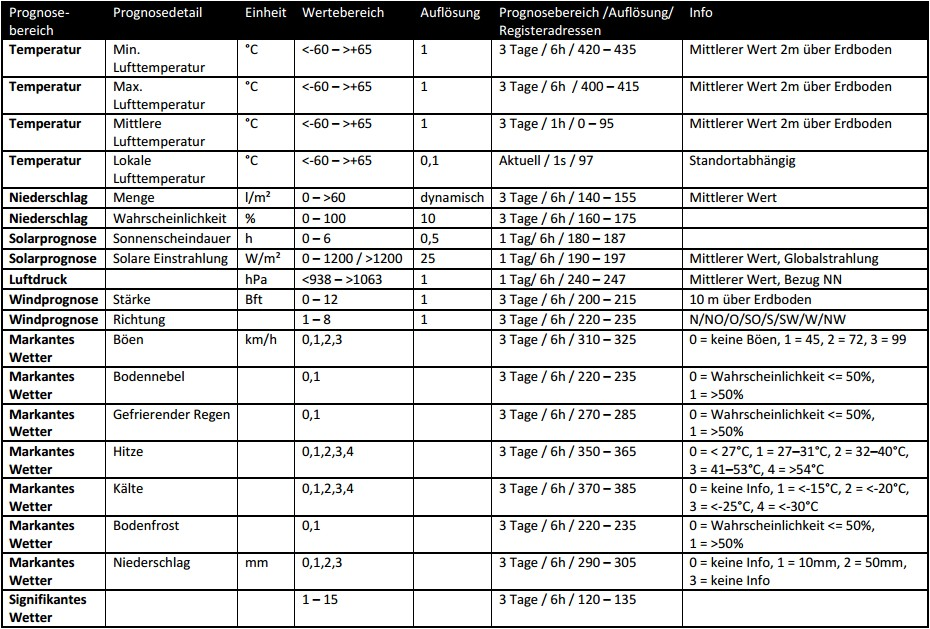
\includegraphics[scale=0.65]{weatherstation/TabDatenstruktur}
%\caption{Detailierte Datenstruktur der Wetterstation\cite[S. 17-26]{HKWDoc}}
%\label{fig:detaildatenstruktur}
%\end{figure}
\begin{table}[!b]
\rotatebox{90}{
\begin{minipage}[!b]{\textwidth}
\resizebox{18.9cm}{!}{ 
\rowcolors{1}{cyan}{white}
{
\setlength{\extrarowheight}{0.1cm}
\begin{tabular}[!b]{| p{2.5cm} | l | l | l | l | l | l | l | p{6.4cm} |}
\hline
\textbf{\parbox[t]{2.7cm}{Prognose-\\Bereich}} & \textbf{Prognosedetail} & \textbf{\parbox[t]{1.2cm}{Ein-\\heit}} & \textbf{Wertebereich} & \textbf{\parbox[t]{1.7cm}{Auf-\\lösung}} & \textbf{\parbox[t]{1.95cm}{Prognose-\\intervall}} & \textbf{\parbox[t]{1.9cm}{zeitliche\\Auflösung}} & \textbf{\parbox[t]{1.9cm}{Register-\\adresse}} & \textbf{Info}\\[1cm]
%\textbf{\parbox[t]{2cm}{Prognose-\\bereich}} & \textbf{Prognosedetail} & \textbf{Einheit} & \textbf{Wertebereich} & \textbf{Aufloesung} & \textbf{Prognoseintervall} & \textbf{zeitliche Aufloesung} & \textbf{Registeradresse} & \textbf{Info}\\[1cm]
\hline \hline
\hiderowcolors
Temperatur & Min. Lufttemperatur & $^\circ$C &  $<-60$ bis $>65$ & 1 & 3 Tage & 6h & 420 - 435 & Mittlerer Wert 2m über Erdboden\\
Temperatur & Max. Lufttemperatur & $^\circ$C &  $<-60$ bis $>65$ & 1 & 3 Tage & 6h & 400 - 415 & Mittlerer Wert 2m über Erdboden\\
Temperatur & Mittlere Lufttemperatur & $^\circ$C &  $<-60$ bis $>65$ & 1 & 3 Tage & 1h & 000 - 095 & Mittlerer Wert 2m über Erdboden\\
Temperatur & Lokale Lufttemperatur & $^\circ$C &  $<-60$ bis $>65$ & 1 & Aktuell & 1s & 097 & Standortabhängig\\
Niederschlag & Menge & l/m$^2$ &  0-60 & dyn. & 3 Tage & 6h & 140 - 155 & Mittlerer Wert\\
Niederschlag & Wahrscheinlichkeit & \% &  0 - 100 & 10 & 3 Tage & 6h & 160 - 175 & \\
Solarprognose & Sonnenscheindauer & h &  0 - 6 & 1 & 1 Tag & 6h & 180 - 187 & Mittlerer Wert\\
Solarprognose & Solare Einstrahlung & W/m$^2$ &  0 – 1200/$>1200$ & 25 & 1 Tag & 6h & 190 - 197 & Mittlerer Wert Globalstrahlung\\
Luftdruck & Min. Lufttemperatur & hPa &  $<938$ – $>1063$ & 1 & 1 Tag & 6h & 240 - 247 & Mittlerer Wert bezogen auf NN\\
Windprognose & Stärke & Bft &  0 - 12 & 1 & 3 Tage & 6h & 200 - 215 & Mittlerer Wert 10m über Erdboden\\
Windprognose & Richtung &  &  1 - 8 & 1 & 3 Tage & 6h & 220 - 235 & N/NO/O/SO/S/SW/W/NW\\
Markantes Wetter & Böen &  &  0,1,2,3 & 1 & 3 Tage & 6h & 310 - 325 & 0=keine Böen, 1=45km/h, 2=72km/h, 3=99km/h \\
Markantes Wetter & Bodennebel &  & 0,1 & 1 & 3 Tage & 6h & 250 - 265 & 0=Wahrscheinlichkeit$<=$50\%, 1=$>$50\%\\
Markantes Wetter & Gefrierender Regen &  & 0,1 & 1 & 3 Tage & 6h & 270 - 285 & 0=Wahrscheinlichkeit$<=$50\%,1=$>$50\%\\
Markantes Wetter & Hitze & $^\circ$C &  0,1,2,3,4 & 1 & 3 Tage & 6h & 350 - 365 & 0=$<$27$^\circ$C, 1=27–31$^\circ$C, 2=32–40$^\circ$C, 3=41–53$^\circ$C, 4=$>$54$^\circ$C\\
Markantes Wetter & Kälte & $^\circ$C &  0,1,2,3,4 & 1 & 3 Tage & 6h & 370 - 385 & 0=keine Info, 1=$<$-15$^\circ$C, 2=$<$-20$^\circ$C, 3=$<$-25$^\circ$C, 4=$<$-30$^\circ$C\\
Markantes Wetter & Bodenfrost &  &  0,1 & 1 & 3 Tage & 6h & 290 - 305 & 0=Wahrscheinlichkeit$<=$50\%, 1=$>$50\%\\
Markantes Wetter & Niederschlag &  &  0,1,2,3 & 1 & 3 Tage & 6h & 330 - 345 & 0=keine Info, 1=10mm, 2=50mm, 3=keine Info\\
Signifikantes Wetter &  &  & 1 - 15 & 1 & 3 Tage & 6h & 120 - 135 & 1=sonnig/klar, 2=leicht bewölkt, 3=vorwiegend bewölkt, 4=bedeckt, 5=Wärmegewitter, 6=starker Regen, 7=Schneefall, 8=Nebel, 9=Schneeregen, 10=Regenschauer, 11=leichter Regen, 12=Schneeschauer, 13=Frontengewitter, 14=Hochnebel, 15=Schneeregenschauer\\
\hline
\end{tabular}
}
}
\caption{Detailierte Datenstruktur der Wetterstation\cite[S. 17-26]{HKWDoc}}
\label{tab:detaildatenstruktur}
\end{minipage}
}
\end{table}
\FloatBarrier
\chapter{Das MODBUS Protokoll}
\begin{figure}[h]
\centering
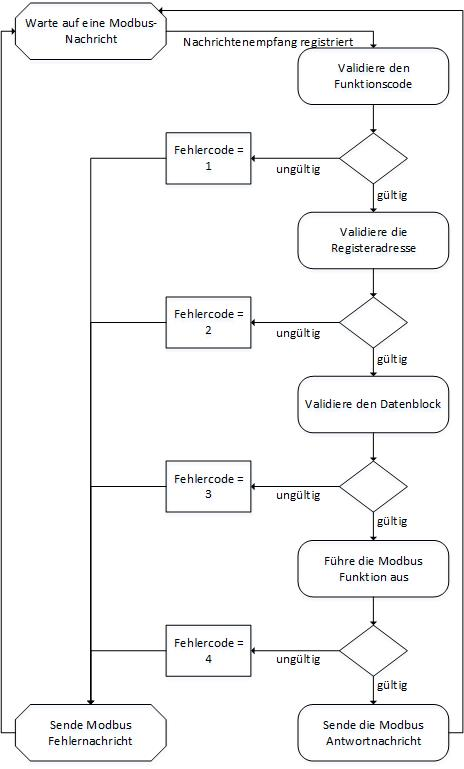
\includegraphics[scale=0.65]{modbus/modbustransdiag}
\caption{Ablaufdiagramm für die MODBUS Nachrichtenüberprüfung \cite[S. 9]{ModbusDoc}}
\label{fig:modbustransdiag}
\end{figure}
\newpage
\begin{figure}[hbtp]
\centering
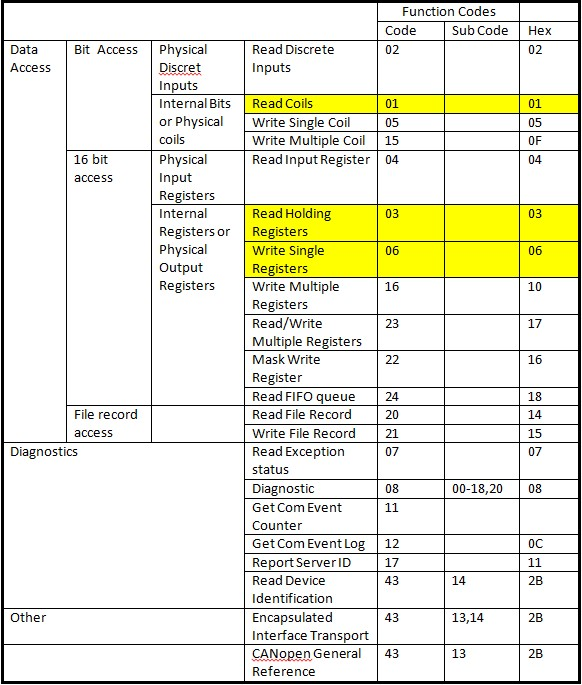
\includegraphics[scale=0.65]{modbus/fcodetab}
\caption{Übersicht der zur Verfügung stehenden Funktionscodes in MODBUS \cite[S. 11]{ModbusDoc}}
\label{fig:fcodetab}
\end{figure} 
\chapter{Hilfsprogramme}

\chapter{Abkürzungsverzeichnis}
\begin{acronym}
\setlength{\parskip}{0ex}
\setlength{\itemsep}{1ex}
 \acro{ADU}{Application Data Unit}
 \acro{Bft}{Beaufort}
 \acro{C}{Celsius}
 \acro{COM}{Communication}
 \acro{CRC}{Cyclic Redundancy Check}
 \acro{DWD}{Deutscher Wetterdienst}
 \acro{EMU}{Energy Management Unit}
 \acro{EV}{Electric Vehicle}
 \acro{FSK}{Frequency Shift Keying}
 \acro{GmbH}{Gesellschaft mit beschränkter Haftung}
 \acro{h}{Stunde}
 \acro{hPa}{Hektopascal}
 \acro{HEMS}{Home Energy Management System}
 \acro{H-Byte}{High-Byte}
 \acro{ID}{Identifkationsnummer}
 \acro{int8}{8 Bit-Integer}
 \acro{IP}{Internet Protocol}
 \acro{I/O}{Input/Output}
 \acro{LMU}{Ludwig-Maximilians-Universität}
 \acro{L-Byte}{Low-Byte}
 \acro{N}{Nord}
 \acro{NN}{Normal Null Meeresspiegel}
 \acro{NO}{Nordost}
 \acro{NW}{Nordwest}
 \acro{O}{Osten}
 \acro{OSI}{Open Systems Interconnection}
 \acro{PDU}{Protocol Data Unit}
 \acro{RMSE}{Root mean square error}
 \acro{RS}{Recommended Standard}
 \acro{RTU}{Remute Terminal Unit}
 \acro{rx}{Empfänger}
 \acro{TCP}{Transmission Control Protocol}
 \acro{S}{Sueden}
 \acro{SO}{Suedost}
 \acro{SW}{Suedwest}
 \acro{W}{Westen}
\end{acronym}
